\documentclass{article}
\usepackage[utf8]{inputenc}
\usepackage[spanish]{babel}
\usepackage{listings}
\usepackage{graphicx}
\graphicspath{ {images/} }
\usepackage{cite}

\begin{document}

\begin{titlepage}
    \begin{center}
        \vspace*{1cm}
            
        \Huge
        \textbf{LA MEMORIA }
            
        \vspace{0.5cm}
        \LARGE
        Nociones de la memoria del computador
            
        \vspace{1.5cm}
            
        \textbf{Mateo Muñoz Arroyave }
            
        \vfill
            
        \vspace{0.8cm}
            
        \Large
        Despartamento de Ingeniería Electrónica y Telecomunicaciones\\
        Universidad de Antioquia\\
        Medellín\\
        Septiembre de 2020
            
    \end{center}
\end{titlepage}

\tableofcontents

\section{Sección introductoria}La memoria es un conjunto de unidades de celdas de almacenamiento asociada a un conjunto de circuitos que se necesitan para ingresar y sacar la información de almacenamiento, se generan un almacenamiento de información binaria en grupos de bits tambien se denominan palabra. Una palabra de memoria es un conjunto de números 1 y 0 que puede representar un número, un codigo o cualquier carácter alfanumérico e información en codigo binario. La capacidad de las memorias por lo general se define como la cantidad total de bytes que pueden almacenar, la mayor parte de las memorias de los computadores utilizan palabras cuyo numero de bits es un múltiplo de 8, es decir, una palabra de 16 bits contiene dos bytes, una de 32 bits contiene cuatro bytes. \\
Se utilizan varios tipos de memoria en los sistemas de computadoras: memoria de acceso aleatorio RAM, memoria de solo lectura ROM, memoria Cache, memoria dinámica DRAM, memoria estática SRAM, memoria Flash, memoria Virtual, memoria de video VRAM.
0

\section{Sección de contenido} \label{contenido}

1.	Defina que es la memoria del computador.
\\

La memoria del computador es uno de los componentes mas fundamentales e importantes en el computador ya que su funcionamiento es almacenar toda la información con la que trabajan todos los microprocesadores para procesarla y entregar los datos que se requieran RAE. \cite{articuloprofe}. Principalmente se divide en dos categorías, memoria principal (RAM y ROM) y memoria secundaria(Disco duro, disco compacto, DVD, Drive, Flash Drive, etc.)
\\
  

2.	Mencione los tipos de memoria y haga una pequeña descripción de cada tipo.\\

RAM: (Random Access Memory) Es la memoria más importante de la computadora ya que se emplea para almacenar temporalmente los datos y toda la información, esta memoria es de escritura y lectura.
\\
ROM: (Read only Memory) Es un chip que almacena en su interior toda la información para poder darle arranque a los dispositivos electrónicos, su función es tener la capacidad de conservar los datos y toda la información sin estar necesariamente alimentada por una fuente de energía, esta memoria cuenta como una de las mas importantes para los dispositivos portátiles o celulares inteligentes.
\\
Cache: Es conocida como memoria de acceso rápido a uno de los recursos mas importantes de una CPU, es donde se almacenan de manera temporalmente todos los datos que fueron procesados recientemente en la memoria auxiliar, su proceso es uno de los mas veloces, existen 3 tipos de cache diferente (L1, L2, L3)
\\
DRAM: (Dynamyc Random Acces Memory) Es la memoria que más ha sido utilizada en las computadoras es una de las más económicas y por ello es una de sus mayores desventajas, su velocidad de proceso es de las más lentas.
\\
SRAM: (Static Random Access memory) Esta memoria está basada en semiconductores, Es capaz de mantener los datos sin necesidad de circuitos de refresco, pierde la información si no esta alimentada por una fuente de energía.
\\
Flash: la memoria flash es un dispositivo que puede almacenar una gran cantidad de datos en un espacio reducido que permite la lectura y escritura de multiples posiciones de memoria en la misma operación.
\\
Virtual: Esta memoria es similar a la cache, es diseñada para ser utilizada exclusivamente por el sistema operativo. A través de este método de memoria el sistema operativo puede disponer de mayor capacidad de memoria de la que ya tiene disponible. 
\\
VRAM: La memoria de video esta presente en las tarjetas gráfica, pero no es igual para todas ellas. La VRAM es un tipo de memoria diseñada especialmente para llevar a cabo un tipo concreto de tarea en aplicaciones graficas y de video.  
\\
3.	Describa la manera como se gestiona la memoria en un computador.
\\
Se trata de proveer mecanismos para asignar secciones de memoria a los programas que las solicitan, y a la vez, liberar las secciones de memoria que ya no se utilizan para que estén disponibles para otros programas. se le llama administrador de memoria y su labor consiste en llevar un registro de las partes de memoria que se estén utilizando y aquellas que no, con el fin de asignar espacio en memoria a los procesos cuando éstos la necesiten y liberándola cuando terminen.  \cite{gestion}
\\
4.	¿Qué hace que una memoria sea más rápida que otra? ¿Por qué esto es importante?
\\

Cada memoria de una computadora tiene un funcionamiento diferente en ella, dependemos de que memoria podríamos hablar, unas son mas veloces que otras pero tienen menos capacidad de almacenamiento que las que son mas lentas y tienen mayor capacidad de almacenamiento, es importante esto porque nos lleva a tener una mejor eficiencia a la hora de funcionar nuestra computadora, cada información que se le escriba o se le pida leer a la computadora va a tener un ciclo de pasos por diferentes tipos de memoria hasta que pueda llegar a una celda del disco duro.
\\
\\


\begin{lstlisting}

\end{lstlisting}

A continuación se presenta un tipo de memoria (\ref{fig:memoria})

\begin{figure}[h]
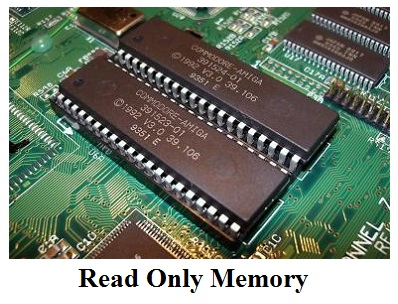
\includegraphics[width=7cm]{memoria.jpg}
\centering
\caption{Memoria}
\label{fig:memoria}
\end{figure}

En la sección de teoremas (\ref{contenido})

\section{Conclusión} \label{conclulsion}
En esta sección podemos aprender y a diferenciar lo importante y lo eficiente que es diferenciar las clases de memoria de una computadora, aca podemos encontrar cada una de las diferencias de las memorias, para que sirve cada una, cual nos debe de funcionar mejor dependiendo de lo que se necesite, nos enseña mucho más de la gestión de los datos y de la información dentro de una memoria.
\bibliographystyle{IEEEtran}
\bibliography{references}

\end{document}
